\chapter{Mapping} \label{chap:mapping}
For accurate foot placement and localisation purposes the robot makes use of two maps, a sparse map covering a large area, and a dense map covering a small
area around the robot. The primarily use of the sparse map is for localisation and extracting pose data, i.e. orientation, velocity and rate. While the dense
map is used to analyse the terrain and find an appropriate point to place the three supporting feet.
It is possible to also use the sparse map for autonomous navigation, however this use case in not covered in this paper.
This chapter covers the design of the mapping system.

The localisation, sparse mapping and pose estimation is handle by ORB-SLAM3 as described in \cite{campos2021orb}. Since ORB-SLAM3 is not a system designed by the author, its
design will not be covered in this chapter. Implementation and operation details will however be covered in chapters \ref{chap:hardware} and \ref{chap:results}.

\section{Projection}
In order to generate a heightmap from a \ac{rgbd} image, it is first required to project the \ac{rgbd} image into 3D space, this is necessary because a heightmap is essentially a 3D environment,
that can be represented as a image due to the assumption of purely convex geometry. 

The camera can be described by its intrinsic and extrinsic parameters. Extrinsic parameters characterise the
cameras position in 3D space, and intrinsic parameters characterise the relationship between the image plane 3D space, 
assuming the camera is at the world origin and an zero rotation. \cite{hartley2003multiple}.

\newpage
\noindent
Refer to figure \ref{fig:projection} as a visual aid regarding projection. Note that this figure is drawn from the perspective of projecting from the image plane into the world,
if the objective was to project from the world onto the image plane the projection center and image plane would swap places, causing the image to be inverted, thus, this figure assumes
that the image rotation has been corrected.
\begin{figure}[h]
    \centering
    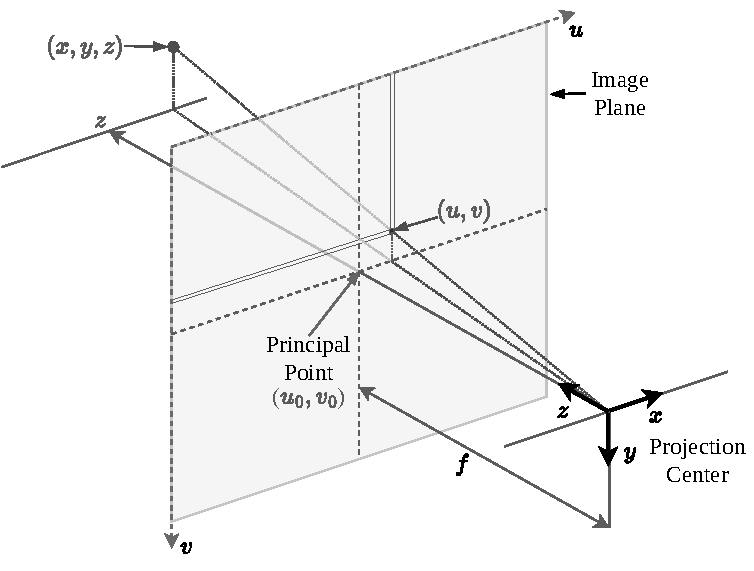
\includegraphics{Diagrams-Projection.drawio.pdf}
    \caption{Camera Projection}
    \label{fig:projection}
\end{figure}

\noindent
Together the extrinsic and intrinsic matrices form the projection matrix,
as shown in equation \ref{eq:projection_matrix},
\begin{equation} \label{eq:projection_matrix}
    \boldsymbol{P} = \boldsymbol{K}
    \begin{bmatrix}
        \boldsymbol{R} & \boldsymbol{T}
    \end{bmatrix}
\end{equation}
where \(\boldsymbol{K}\) is the intrinsic matrix and \(\begin{bmatrix} \boldsymbol{R} & \boldsymbol{T} \end{bmatrix}\) the extrinsic matrix, these are described
in equation \ref{eq:intrinsic} and \ref{eq:extrinsic}.

The projection matrix can be used to project a point on the projection plane into world space as shown in equation \ref{eq:full_projection}.

\begin{equation} \label{eq:full_projection}
    \begin{bmatrix}
        u \\
        v \\
        1
    \end{bmatrix}
    = \boldsymbol{P}
    \begin{bmatrix}
        x \\
        y \\
        z \\
        1
    \end{bmatrix}
\end{equation}
where \(u,v\) are the pixel coordinates on the projection plane and \(x,y,z\) are the coordinates in world space.
\begin{equation} \label{eq:intrinsic}
    \boldsymbol{K} =
    \begin{bmatrix}
        \alpha_x & \gamma   & u_0 \\
        0        & \alpha_y & v_0 \\
        0        & 0        & 1
    \end{bmatrix}
\end{equation}
where the focal length is represented by,
\[\alpha_x = f \cdot m_y\]
\[\alpha_y = f \cdot m_x\]
with \(m_x\) and \(m_y\) being the inverse of the width and height of a projection plane pixel, \(f\) the focal length and \(u_0\),\(v_0\) being the principal point, optimally the center of the projection plane.
The skew coefficient, \(\gamma\), is often (and in this case) 0.

The extrinsic matrix is as shown below,
\begin{equation}\label{eq:extrinsic}
    \begin{bmatrix}
        \boldsymbol{R} & \boldsymbol{T}
    \end{bmatrix}
    =
    \begin{bmatrix}
        \boldsymbol{R}_{3\times3} & \boldsymbol{T}_{3\times1} \\
        \boldsymbol{0}_{1\times3} & 1
    \end{bmatrix}
\end{equation}
where \(\boldsymbol{R}\) characterises the camera's heading in world space and \(\boldsymbol{T}\) the world origin expressed in 
the camera coordinate frame.

For ease of preprocessing points are first projected into the camera coordinate frame, in other words, the extrinsic matrix is omitted from equation \ref{eq:full_projection}.
The resultant matrix equation is shown in equation \ref{eq:local_projection}.

\begin{equation} \label{eq:local_projection}
    \begin{bmatrix}
        u \\
        v \\
        1 \\
        1/z
    \end{bmatrix}
    = \frac{1}{z}
    \begin{bmatrix}
        f_x & 0 & c_x & 0 \\
        0 & f_y & c_y & 0 \\
        0 & 0 & 1 & 0 \\
        0 & 0 & 0 & 1
    \end{bmatrix}
    \begin{bmatrix}
        x\\
        y\\
        z\\
        1
    \end{bmatrix}
\end{equation}
From equation \ref{eq:local_projection} \(x,y,z\) are found to be show in equation \ref{eq:proj_z} to \ref{eq:proj_y}.
\begin{align}
    z &= D_{u,v} \label{eq:proj_z}\\[0.2cm]
    x &= \frac{z(u - u_0)}{\alpha_x}\label{eq:proj_x} \\
    y &= \frac{z(v - v_0)}{\alpha_y}\label{eq:proj_y}
\end{align}
where \(D_{u,v}\) is the depth image pixel value at pixel coordinate \(u,v\).


\section{Memory}

